\documentclass[notheorems, handout]{beamer}

\usetheme[numbers,totalnumbers,compress, nologo]{Statmod}
\usefonttheme[onlymath]{serif}
\setbeamertemplate{navigation symbols}{}
\setbeamertemplate{theorems}[numbered]
\setbeamertemplate{caption}[numbered]

\mode<handout> {
	\usepackage{pgfpages}
	\setbeameroption{show notes}
	\pgfpagesuselayout{2 on 1}[a4paper, border shrink=5mm]
	\setbeamercolor{note page}{bg=white}
	\setbeamercolor{note title}{bg=gray!10}
	\setbeamercolor{note date}{fg=gray!10}
}

\usepackage[utf8x]{inputenc}
\usepackage[T2A]{fontenc}
\usepackage[russian]{babel}
\usepackage{tikz}
\usepackage{ragged2e}
\usepackage{amsmath,amssymb}
\usepackage{graphicx}
\usepackage{caption}
\usepackage{subcaption}
\usepackage{color}
\usepackage{dcolumn}
\usepackage{bm}
\usepackage{float}
\usepackage[authoryear]{natbib}
%\usepackage[numbers, sort&compress]{natbib}


\newtheorem{corollary}{Следствие}
\newtheorem{theorem}{Теорема}
\newtheorem{remark}{Замечание}
\newtheorem{comment}{Замечание} % задаём выводимое слово (для определений)
\newtheorem{lemma}{Лемма}
\newtheorem{sentence}{Предложение}
\newtheorem{definition}{Определение}
\newtheorem{formulation}{Формулировка}
\newtheorem{statement}{Постановка}
\DeclareMathOperator{\R}{\mathbb{R}}
\DeclareMathOperator{\rank}{\mathrm{rank}}
\newcommand{\norm}[1]{\left\|#1\right\|}

\newcommand{\SSA}{\textbf{SSA}}
\newcommand{\CISSA}{\textbf{CiSSA}}
\newcommand{\TS}{\mathsf{X}}



\title[Модификации метода $\SSA$]{Модификации метода анализа сингулярного спектра для анализа временных рядов: Circulant SSA}

\author{Погребников Николай Вадимович, гр. 21.Б04-мм}

\institute[Санкт-Петербургский Государственный Университет]{%
	\small
	Санкт-Петербургский государственный университет\\
	Прикладная математика и информатика\\
	Вычислительная стохастика и статистические модели\\
	\vspace{1.25cm}
	3 курс (бак.) <<Производственная практика (научно-исследовательская работа)>>\\(Семестр 6)}

\date[Зачет]{Санкт-Петербург, 2024}

\subject{Talks}

\begin{document}
%	\begin{frame}[plain]
%		\titlepage
%		
%		\note{Научный руководитель  к.ф.-м.н., доцент Некруткин В.В.,\\
%			кафедра статистического моделирования\\\vspace*{2cm}\emph{Моя отметка за работу Дениса Яковлева -- 5  с минусом (очень хорошо).
%				5 за результат, минус – за стиль работы.
%		}}
%	\end{frame}
	\begin{frame}[plain]
		\titlepage
		
		\note{Научный руководитель  д.\,ф.-м.\,н., доц. Голяндина Нина Эдуардовна,\\
			кафедра статистического моделирования}
	\end{frame}
	
	%\section{Короткая тема}
	%\subsection{Общие слова}
	
%	\setbeameroption{show notes}
	
	\begin{frame}{Введение}
		Временные ряды представляют собой последовательность данных, собранных или
		измеренных в хронологическом порядке. Понимание эволюции явлений во времени является критическим для выявления тенденций, циклов и аномалий. В этих целях были созданы методы разложения временных рядов на сумму интерпретируемых компонент такие как $\SSA$ \citep{golyandina2001analysis} и его модификация $\CISSA$ \citep{bogalo2020}.
		
		
		Перед началом исследования были поставлены следующие цели:
		\begin{enumerate}
			\item Ознакомиться с алгоритмом $\CISSA$;
			\item Реализовать алгоритм $\CISSA$ на языке R; 
			\item Сравнить алгоритмы $\SSA$, разложение Фурье и $\CISSA$.
		\end{enumerate}
		%		Задача --- оценка ошибок восстановления ряда.
		%		Тут какое-то введение.
		%		Что за задача решается, какое метод используется, какая цель работы.
		
		\note{
			Сингулярный спектральный анализ ($\SSA$ \citep{golyandina2001analysis}) --- метод, целью которого является разложение оригинального ряда на сумму небольшого числа интерпретируемых компонент, таких как медленно изменяющаяся тенденция (тренд), колебательные компоненты (сезонность) и ``структурный'' шум.  В данном исследовании
			рассматривается математическая составляющая вариации алгоритма $\SSA$ --- circulant singular spectrum analysis ($\CISSA$), предложенная в статье \citep{bogalo2020}, а также сравнение базового метода и циркулярного, применение их на языке R.
		}
	\end{frame}
	
	
	
	\begin{frame}{Метод SSA. Алгоритм: разложение}
		Для временного ряда $\TS = (x_1, \dots, x_{N})$ выбирается длина окна $L$, $1 < L < N$ и определяется $K = N - L + 1$. Строится L-траекторная матрица $\mathbf{X}$, состоящая из столбцов вида $\TS_i = ( x_{i-1}, \ldots, x_{i+L-2})^{\mathrm{T}}$,
		$1 \leq i \leq K$. \\
		
		
		Пусть $\mathbf{S} = \mathbf{X}\mathbf{X}^{\mathrm{T}}$, 
		$\lambda_1, \dots, \lambda_L$ --- собственные числа матрицы $\mathbf{S}$, взятые в неубывающем порядке. \\
		\begin{definition}
			Сингулярным разложением называется представление матрицы в виде:
			\begin{equation}
				\mathbf{X} = \mathbf{X}_1 + \dots + \mathbf{X}_d =
				\sum_{i = 1}^{d} \sqrt{\lambda_i} U_i V_{i}^{\mathrm{T}}\label{eq:u},
				\text{где}
			\end{equation}
			
			$U_1, \dots, U_L$ --- ортонормированная система собственных векторов матрицы $\mathbf{S}$, $d = \max{ \{i: \lambda_i > 0 \}}$ и 
			$V_i = \mathbf{X}^{\mathrm{T}} U_i / \sqrt{\lambda_i}$.
		\end{definition}
		
		\note{
			Полезным свойством является то, что матрица $\mathbf{X}$ имеет одинаковые элементы на антидиагоналях. Таким образом, $L$-траекторная матрица является ганкелевой.
			
			Набор $( \sqrt{\lambda_i}, U_i, V_{i}^{\mathrm{T}})$ называется $i$-й собственной тройкой разложения $\mathbf{X}$.
		}
	\end{frame}


	\begin{frame}{Метод SSA. Алгоритм: восстановление}
		На основе разложения \eqref{eq:u} производится процедура группировки, которая делит все множество индексов $\{1, \dots, d\}$ на $m$ непересекающихся подмножеств $I_1, \dots, I_d$. \\
		Пусть $I = \{i_1, \dots, i_p\}$, тогда $\mathbf{X}_I =
		\mathbf{X_{i_1}} + \dots + \mathbf{X_{i_p}}$. Такие матрицы вычисляются для каждого $I = I_1, \dots, I_m$. \newline \newline \pause
		В результате получаются матрицы $\mathbf{X_{I_1}}, \dots, \mathbf{X_{I_m}}$, для каждой из которых проводится операция диагонального усреднения, составляющая ряды длины $N$: $\TS_1, \dots, \TS_m$. \\ 
		При этом, $\TS_1 + \dots + \TS_m = \TS$.
		
		\note{
			Диагональное усреднение для каждой антидиагонали усредняет значения элементов матрицы.
			
			Применяя данную операцию к матрицам $\mathbf{X_{I_1}}, \dots, \mathbf{X_{I_m}}$, получаются $m$ новых рядов: $\TS_1, \dots, \TS_m$. При этом, $\TS_1 + \dots + \TS_m = \TS$.
		}
		
		
	\end{frame}
	
	
	\begin{frame}{Метод SSA. Свойства: точная разделимость}
		Пусть временной ряд  $\TS = \TS^{(1)} + \TS^{(2)}$ и задачей является нахождение этих слагаемых.
		
		Будем говорить, что ряд $\TS$ точно разделим на $\TS^{(1)} $ и $ \TS^{(2)}$, если существует такое сингулярное разложение траекторной матрицы $\mathbf X$ ряда $\TS$, что его можно разбить на две части, являющиеся сингулярными разложениями траекторных матриц рядов $\TS^{(1)}, \TS^{(2)}$ \citep{golyandina2001analysis}.
		
		
		
		
		\note{
			Условия точной разделимости выводятся из понятий слабо L-разделимых рядов и сильно L-разделимых рядов \citep{golyandina2001analysis}. Стоит отметить, что точная разделимость для $\cos$ достигается, если $Lw \in \mathbb{N}, \, Kw \in \mathbb{N}$, где $w$ --- частота.
			
			Однако условия точной разделимости достаточно жесткие и вряд ли выполнимы в реальных задачах. Тогда появляется такое понятие, как асимптотическая разделимость.
		}
		
		
	\end{frame}
	
	
	
	\begin{frame}{Метод SSA. Свойства: асимптотическая разделимость}
		
		\begin{equation*}
			\rho_{i,j}^{(M)}=\frac{\left(\TS_{i,i+M-1}^{(1)},\TS_{j,j+M-1}^{(2)}\right)}{\left|\left|\TS_{i,i+M-1}^{(1)}\right|\right|\left|\left|\TS_{j,j+M-1}^{(2)}\right|\right|}.
		\end{equation*}
		
		\begin{definition}
			Ряды $\TS^{(1)}, \TS^{(2)}$ называются $\varepsilon$-разделимыми при длине окна $L$, если
			\begin{equation*}
				\rho^{(L,K)}\ {\stackrel{\mathrm{def}}{=}}\ \mathrm{max}\left(\operatorname*{max}_{1\leq i,j\leq K}|\rho_{i,j}^{(L)}|,\operatorname*{max}_{1\leq i,j\leq L}|\rho_{i,j}^{(K)}|\right)<\varepsilon
				\text{  .}
			\end{equation*}
			
		\end{definition}
		
		\begin{definition}
			Если $\rho^{(L(N),K(N))} \rightarrow 0$ при некоторой последовательности $L = L(N) $, $N \rightarrow \infty$, то ряды $\TS^{(1)}, \TS^{(2)}$ называются асимтпотически $L(N)$-разделимыми \citep{golyandina2001analysis}.
		\end{definition}
		
		\note{
			Для любого ряда $\TS$ длины $N$ определим
			$\TS_{i,j}\,=\,(x_{i-1},\cdot\cdot\cdot,x_{j-1}),\;\;1\,\leq\,i\,\leq\,j\,<\,N.$
			Пусть $\TS^{(1)}=(x_{0}^{(1)},\ldots,x_{N-1}^{(1)}),\TS^{(2)}=(x_{0}^{(2)},\ldots,x_{N-1}^{(2)}).$ Тогда определим коэффициент корреляции.
			
		}
		
		
	\end{frame}
	
	
	\begin{frame}{Метод SSA. Свойства: асимптотическая разделимость}
		
		
		
		\begin{comment}
			Для $\SSA$ существуют алгоритмы улучшения разделимости \citep{golyandina2023intelligent}. Они позволяют более точно отделять временные ряды друг от друга. В данной работе будут использоваться методы EOSSA и FOSSA.
		\end{comment}
		
		\note{
			Для нас важно, что благодаря применению улучшения разделимости мы можем делать автоматическую группировку по заданным частотам в базовом алгоритме $\SSA$.
		}
		
		
	\end{frame}
	
	
	
	\begin{frame}{Метод CiSSA. Алгоритм: разложение}
		Как и в $\SSA$ считается $\mathbf X$, по которой строится $\hat{\mathrm{C}}_{L}$:
		$\hat c_m = \frac{L-m}{L}\hat{\gamma}_m + \frac{m}{L}\hat{\gamma}_{L-m}$, $ \hat{\gamma}_m = \frac{1}{N-m} \sum \limits_{t = 1}^{N-m}x_t x_{t+m}$, $ \, m = 0:L-1$.
		\begin{equation*}
			\label{eq:circ_mat}
			\hat{\mathrm{C}}_{L}=\left(\begin{array}{cccc}
				\hat c_{1} & \hat c_{2} & \ldots & \hat c_{L} \\
				\hat c_{2} & \hat c_{1} & \ldots & \hat c_{L-1} \\
				\vdots & \vdots & \vdots & \vdots \\
				\hat c_{L} & \hat c_{L-1} & \hdots & \hat c_{1}
			\end{array}\right).
		\end{equation*}
		Собственные числа и вектора матрицы $\hat{\mathrm{C}}_{L}$, задаются по формулам:
		\begin{equation*}
			\begin{split}
				&U_{k}=L^{-1/2}(u_{k,1\cdot}\cdot\cdot\cdot,u_{k,L}), \, \text{где} \, 
				u_{k,j}=\exp\left(-\mathrm{i}2\pi\d(j-1)\frac{k-1}{L}\right), \\
				&\lambda_{L,k}=\sum_{m=0}^{L-1}\hat c_{m}\exp\left(i 2\pi m\frac{k-1}{L}\right), \, k = 1:L.
			\end{split}
		\end{equation*}
		
		\note{
			Модификация $\SSA$ на основе циркулярной матрицы \citep{bogalo2020}. Авторы метода называют её автоматизированной. Причем автоматизированная в том смысле, что компоненты ряда группируются по частотам самим алгоритмом.
		}
		
	\end{frame}
	
	
	
	\begin{frame}{Метод CiSSA. Алгоритм: восстановление}
		Для каждой частоты $w_k = \frac{k-1}{L}$, $k = 2:\lfloor \frac{L+1}{2} \rfloor$, есть два собственных вектора: $U_k$ и $U_{L+2-k}$. За частоту $w_0$ отвечает один собственный вектор --- $U_0$. Если $L$ --- четное, то частоте $w_{\frac{L}{2} + 1}$ будет соответствовать один вектор $U_{\frac{L}{2}+1}$.
		
		Следовательно, индексы разбиваются на элементарную группировку следующим образом:
		\begin{equation*}
			\begin{split}
				&B_1 = \{1\}; \, B_k = \{k, L+2-k\}, \,  \text{для } k = 2:\lfloor \frac{L+1}{2}\rfloor; \\ \, 
				&B_{\frac{L}{2} + 1} = \left\{ \frac{L}{2} + 1 \right\}, \, \text{если} \, L \mid  2.
			\end{split}
		\end{equation*}
		$\mathbf X_{B_k} = \mathbf X_k + \mathbf X_{L+2-k} = U_k U_k^H \mathbf X + U_{L+2-k} U_{L+2-k}^H \mathbf X$, \\где $U^H$ --- это комплексное сопряжение и транспонирование вектора $U$. Далее идет группировка по диапазонам интересующих частот, после чего следует диагональное усреднение.
		
		\note{
			Группировка будет производиться на непересекающиеся подгруппы по частотам от $0$ до $0.5$, поскольку частоты выше 0.5 представляют собой зеркальное отражение частот ниже 0.5. Именно поэтому объединяются матрицы $\mathbf X_{B_k} = \mathbf X_k + \mathbf X_{L+2-k}$.
		}
		
	\end{frame}
	
	
	
	\begin{frame}{Метод CiSSA. Свойства: связь с разложением Фурье}
		\begin{definition}
			Разложение
			\begin{equation}
				\label{eq:fourier}
				x_n = c_0 + \sum\limits_{k = 1}^{\lfloor \frac{N+1}{2} \rfloor}\left(c_k \cos(2\pi n k / N) + s_k \sin(2\pi n k / N) \right),
			\end{equation}
			где $1 \leq n \leq N$ и $s_{N/2} = 0 $ для четного N, называется разложением Фурье ряда $\TS$. 
		\end{definition}
		\begin{comment}
			\label{comm:proector}
			$U_k U_k^H + U_{L+2-k} U_{L+2-k}^H$ является оператором проектирования на подпространство, которое порождено синусами и косинусами с частотой $w_k = \frac{k-1}{L}$. Это пространство соответствует компонентам синусоидальной структуры временного ряда, связанных с конкретной частотой, выделяемой методом. 
		\end{comment}
		\note{
			По замечанию \ref{comm:proector} видно, что при вычислении $\mathbf X_{B_k} = \mathbf X_k + \mathbf X_{L+2-k} = U_k U_k^H \mathbf X + U_{L+2-k} U_{L+2-k}^H \mathbf X$, воспроизводится разложение Фурье для $K$ векторов матрицы $\mathrm X$. Затем вычисляется диагональное усреднение $\mathbf *X_{B_k}$.
		}
		
	\end{frame}
	
	\begin{frame}{Метод CiSSA. Свойства: разделимость}
		\textbf{Точная разделимость.}
		Поскольку данный метод является аналогом разложения Фурье, то в смысле сильной разделимости можно точно разделить ряд, в котором одной из компонентов является $\cos(2\pi w + \varphi)$ с частотой $w$ такой, что $Lw = k \in \mathbb N$, или константа.
		
		\textbf{Асимптотическая разделимость.} 
		\begin{definition}
			Пусть $\TS = \TS^{(1)} + \TS^{(2)}$. Существуют такие диапазоны частот $I_1$ и $I_2$ и последовательность $L = L(N) $, $N \rightarrow \infty$, что при них $\mathrm{MSE}\left(\TS^{(1)}, \TS^{(1)}_{\CISSA}\right) \rightarrow 0$ и $\mathrm{MSE}\left(\TS^{(2)}, \TS^{(2)}_{\CISSA}\right) \rightarrow 0$, где $MSE$ --- среднеквадратическая ошибка, $\TS^{(1)}_{\CISSA}$ и $ \TS^{(2)}_{\CISSA}$ компоненты ряда, полученные алгоритмом $\CISSA$ для частот $I_1$ и $I_2$, то ряды $\TS^{(1)}$ и $ \TS^{(2)}$ называются $\CISSA$-асимтпотически $L(N)$-разделимыми.
		\end{definition}
		
		\note{
			Асимптотическая разделимость в данном случае будет означать, что при увеличении $L$ разбиение сетки будет увеличиваться, а значит, и частоты в сетке начнут сближаться к истинным частотам периодических компонентов (либо становиться равными им), что будет снижать ошибку вычислений.
		}
		
	\end{frame}
	
	
	\begin{frame}{Метод CiSSA. Свойства: эквивалентность методов}
		\begin{definition}
			Будем говорить, что методы $M_1$ и $M_2$ асимптотически эквивалентны, если их матрицы вложения $S_1$, $S_2$ асимптотически эквиваленты в смысле $\operatorname*{lim}\limits_{L\rightarrow\infty \, N\rightarrow\infty}\frac{||{S_1-S_2}||_F}{\sqrt{L}}=0$, при некоторой последовательности $L = L(N) $, $N \rightarrow \infty$, где $||{\cdot}||_F$ --- норма Фробениуса. Тогда $M_1 \sim M_2$, $S_1 \sim S_2$.
		\end{definition}
		
		
		\begin{theorem}
			\label{th:equiv}
			Дана $L \times K$ траекторная матрица $\mathbf{X}$. Пусть $S_B = \mathbf{X} \mathbf{X}^T / K$, $S_C$ --- матрица, определенная в \eqref{eq:circ_mat}. Тогда $S_B \sim S_C$.
		\end{theorem}
		\begin{proof}
			Доказательство в источнике \citep{bogalo2020}.
		\end{proof}
		
		\note{
			В статье \citep{bogalo2020} говорится, что асимптотически методы $\SSA$ и $\CISSA$ эквивалентны и в доказательство приводится теорема.
		}
		
	\end{frame}
	
	\begin{frame}{Метод CiSSA. Свойства: применимость к нестационарным рядам}
		Алгоритм $\CISSA$, описанный ранее, изначально применим только к стационарным временным рядам. Однако, как утверждается авторами статьи \citep{bogalo2020}, для использования на нестационарных временных рядах, нужно выполнить расширение ряда.  Эта процедура позволяет предсказать значения временного ряда за его пределами (экстраполяция) как в правом, так и в левом направлениях на заданное число шагов $H$.
		Таким образом, трендовая (нелинейная) компонента ряда будет выделяться заметно лучше.
		
		
		\note{
			Формальное определение стационарности ряда можно увидеть в отчёте данной работы \citep{spbu_cissa_coursework_github}. Стационарный ряд --- это такой временной ряд, в котором изменения происходят вокруг некоторого среднего значения, и это среднее остаётся более-менее постоянным на протяжении всего ряда.
			
			Сама процедура расширения ряда $\TS$ производится с использованием авторегрессионной (AR) модели.
		}
		
		
	\end{frame}
	
	\begin{frame}{Сравнение алгоритмов. SSA, разложение Фурье, CiSSA }
		Для начала будем рассматривать разделимость рядов без шума, затем с шумом.
		В сравнении будут присутствовать пять различных методов: базовый $\SSA$,  $\SSA$ с использованием EOSSA для улучшения разделимости, разложения Фурье, базового $\CISSA$ и $\CISSA$ с расширением ряда. Для наглядного отображения преимуществ каждого из этих методов составлена таблица \ref{tab:advantages}.
		\begin{table}[H]
			\centering
			\tiny
			\begin{center}
				\begin{tabular}{ccccccccc}
					\hline
					Метод/Условие  &|& $\cos$,                 & $\cos$,                    & $\cos$,                     & $\TS_{\mathrm{np1}}$   & $\TS_{\mathrm{np}}$ & group\\ 
					&|& $Lw = k \in \mathbb N$, & $Lw = k \in \mathbb N$,    & $Lw = k \not\in \mathbb N$, &             \\
					&|& $Kw = k \in \mathbb N$  & $Kw = k \not\in \mathbb N$ & $Kw = k \not\in \mathbb N$  &             \\ 
					\hline
					SSA            &|& $+$                     & $\to$                      & $\to$                       & $\to$ & $\to$ & $-$ \\
					SSA EOSSA      &|& $+$                     & $\to$                      & $\to$                       & $\to$ & $\to$ & $+$ \\
					Fourier        &|& $+$                     & $+$                        & $\to$                       & $-$   & $-$ & $+$ \\
					CiSSA          &|& $+$                     & $+$                        & $\to$                       & $-$   & $-$ & $+$ \\
					CiSSA extended &|& $+$                     & $+$                        & $\to$                       & $\to$ & $-$ & $+$ \\
					\hline
				\end{tabular}
			\end{center}
			\caption{Преимущества и недостатки ряти методов} 
			\label{tab:advantages}
		\end{table}
		
		\note{
			На пересечении строк и столбцов указан знак, показывающий, достигается ли разделение компоненты: плюс (+) обозначает точное выполнение, знак стремления указывает на асимптотическое выполнение, а минус (–) --- на отсутствие разделимости. Для разложения Фурье подразумевается, что $L = N$. 
			
			Обозначения: 
			\begin{itemize}
				\item $\cos$ --- в ряде присутствуют только периодические компоненты вида $\cos(2\pi\omega x + \varphi)$;
				\item $\TS_{\mathrm{np}1}$ --- одна непериодическая компонента в ряде, остальные имеют период;
				\item $\TS_{\mathrm{np}}$ --- несколько непериодических компонент в ряде, остальные имеют период, интересует разделение между
				непериодическими компонентами;
				\item group --- автоматическая группировка по заданным частотам.
			\end{itemize}
		}
		
		
		
	\end{frame}
	
	
	\begin{frame}{Сравнение алгоритмов. Пример 1 }
		$\TS = \TS_{\sin} + \TS_{\cos} = \sin{\frac{2\pi}{12}x} + \frac{1}{2}\cos{\frac{2\pi}{3}x}$, $L = 96$, $N = 96 \cdot 2$ для разложения Фурье и $N = 96 \cdot 2 - 1$ для остальных, чтобы выполнялись условия выполнения разделимости частот. Сравним результаты по среднеквадратичной ошибке:
		
		\begin{table}[H]
			\centering
			\begin{tabular}{llllllll}
				\hline
				Метод/Компонента & $\TS_{\sin}$ & $\TS_{\cos}$ \\ 
				\hline
				SSA & 6.8e-30 & 1.5e-29 \\ 
				SSA EOSSA & 1.5e-29 & 7.5e-30 \\ 
				Fourier & 1.7e-28 & 3.5e-28 \\ 
				CiSSA & 1.9e-29 & 5.3e-30 \\ 
				CiSSA extended & 2.0e-04 & 8.6e-04 \\ 
				\hline
			\end{tabular}
			\caption{MSE разложений ряда $\TS = \TS_{\sin} + \TS_{\cos}$ пяти методов} 
			\label{tab:errs_fourier_cissa_sin_cos}
		\end{table}
		
		
		\note{
			Таблица \ref{tab:errs_fourier_cissa_sin_cos} показывает, что первые четыре разложения сделали правильное (с точностью до вычислений с помощью компьютера) разделение компонент ряда. Однако расширение в методе $\CISSA$ ухудшило разделимость периодических частей.
		}
		
		
	\end{frame}
	
	\begin{frame}{Сравнение алгоритмов. Пример 2 }
	$\TS = \TS_{\sin} + \TS_{\cos} + \TS_{\mathrm{noise}} = \sin{\frac{2\pi}{12}x} + \frac{1}{2}\cos{\frac{2\pi}{3}x} + \varepsilon_n$, где $\varepsilon_n \sim \mathrm N(0, 0.1)$, $L = 96$, $N = 96 \cdot 2$ для разложения Фурье и $N = 96 \cdot 2 - 1$ для остальных.
		
		\begin{table}[H]
			\centering
			\begin{tabular}{llllllll}
				\hline
				Метод/Компонента & $\TS_{\sin}$ & $\TS_{\cos}$ \\ 
				\hline
				SSA & 2.9e-04 & 3.1e-04 \\ 
				SSA EOSSA & 2.9e-04 & 3.1e-04 \\ 
				Fourier & 1.0e-04 & 1.1e-04 \\ 
				CiSSA & 1.6e-04 & 1.8e-04 \\ 
				CiSSA extended & 6.6e-04 & 1.9e-03 \\ 
				\hline
			\end{tabular}
			\caption{MSE разложений ряда $\TS = \TS_{\sin} + \TS_{\cos} +\TS_{\mathrm{noise}}$ пяти методов} 
			\label{tab:errs_fourier_cissa_sin_cos_noised}
		\end{table}
		
		
		\note{
			Проводилось $100$ тестов, в таблице \ref{tab:errs_fourier_cissa_sin_cos_noised} указаны средние значения ошибки для одних и тех же реализаций шума.
			
			Был проведен парный t-критерий для зависимых выборок с целью проверки гипотезы о равенстве средних значений ошибки для каждой компоненты, попарно для всех методов. В качестве нулевой гипотезы ($H_0$) предполагалось, что средние значения двух сравниваемых выборок равны. Критический уровень значимости был установлен на уровне $\alpha = 0.05$.
			Результаты анализа показали, что во всех случаях $p$-значение оказались меньше 0.05, что позволяет отвергнуть нулевую гипотезу.
		}
		
		
	\end{frame}
	
	
	\begin{frame}{Сравнение алгоритмов. Пример 3 }
		$\TS = \TS_{\sin} + \TS_{\cos} + \TS_{c} + \TS_e = \sin{\frac{2\pi}{12}x} + \frac{1}{2}\cos{\frac{2\pi}{3}x} + 1 + e^{\frac{x}{100}}$, $L = 96$, $N = 96 \cdot 2$ для разложения Фурье и $N = 96 \cdot 2 - 1$
		
		\begin{table}[H]
			\centering
			\begin{tabular}{llllllll}
				\hline
				Метод/Компонента & $\TS_{c} + \TS_e$ & $\TS_{\sin}$ & $\TS_{\cos}$ \\ 
				\hline
				SSA & 5.0e-03 & 8.9e-07 & 5.2e-05 \\ 
				SSA EOSSA & 1.7e-28 & 1.6e-29 & 8.7e-30 \\ 
				Fourier & 1.1e-01 & 6.1e-04 & 6.8e-03 \\ 
				CiSSA & 5.3e-02 & 1.6e-05 & 4.9e-04 \\ 
				CiSSA extended & 5.0e-04 & 2.1e-04 & 1.1e-03 \\ 
				\hline
			\end{tabular}
			\caption{MSE разложений ряда $\TS = \TS_{\sin} + \TS_{\cos} + \TS_{c} + \TS_e$ четырех методов} 
			\label{tab:errs_fourier_cissa_trend}
		\end{table}
		
		
		\note{
			Непериодические компоненты будут отвечать низким частотам. Проблема лишь в том, что с помощью методов разложения Фурье $\CISSA$ невозможно различить между собой две непериодические компоненты, поскольку группировка работает по частотам, элементы разложения неизбежно смешаются между собой. Будем искать экспоненту и константу по низким частотам, назовем это трендовой составляющей ряда. По таблице \ref{tab:advantages} лучше всех должен справиться $\SSA$ с улучшением разделимости EOSSA. Хуже всех --- разложение Фурье, поскольку он никаким образом не сможет вычленить из ряда экспоненту.
			
			Результаты таблицы \ref{tab:errs_fourier_cissa_trend} повторяют вышеизложенные рассуждения. Также заметно, что периодические компоненты лучше выделились с помощью $\CISSA$ без процедуры расширения ряда в сравнении с $\CISSA$ с расширением.
		}
		
		
	\end{frame}
	
	
	\begin{frame}{Сравнение алгоритмов. Пример 4 }
		$\TS = \TS_{\sin} + \TS_{\cos} + \TS_{c} + \TS_e + \TS_{\mathrm{noise}} = \sin{\frac{2\pi}{12}x} + \frac{1}{2}\cos{\frac{2\pi}{3}x} + 1 + e^{\frac{x}{100}} +  + \varepsilon_n$, где $\varepsilon_n \sim \mathrm N(0, 0.1)$, $L = 96$, $N = 96 \cdot 2$ для разложения Фурье и $N = 96 \cdot 2 - 1$.
		
		\begin{table}[H]
			\centering
			\begin{tabular}{llllllll}
				\hline
				Метод/Компонента & $\TS_{\sin}$ & $\TS_{\cos}$ & $\TS_{c} + \TS_e$\\ 
				\hline
				SSA & 2.9e-04 & 3.6e-04 & 5.2e-03 \\ 
				SSA EOSSA & 2.9e-04 & 3.1e-04 & 9.4e-04 \\ 
				Fourier & 6.9e-04 & 7.2e-03 & 1.2e-01 \\ 
				CiSSA & 1.7e-04 & 7.0e-04 & 5.5e-02 \\ 
				CiSSA extended & 6.8e-04 & 2.1e-03 & 2.7e-03 \\ 
				\hline
			\end{tabular}
			\caption{MSE разложений ряда $\TS = \TS_{\sin} + \TS_{\cos} + \TS_{c} + \TS_e+\TS_{\mathrm{noise}}$ четырех методов} 
			\label{tab:errs_fourier_cissa_trend_noised}
		\end{table}
		
		
		\note{
			Как видно из таблицы \ref{tab:errs_fourier_cissa_trend_noised}, разделения ухудшились, однако $\SSA$ с улучшением разделимости EOSSA отработал лучше всех. Также был проведен был проведён двухвыборочный t-критерий для зависимых выборок с целью проверки гипотезы о равенстве средних значений ошибки для каждой компоненты, попарно для всех методов. В качестве нулевой гипотезы ($H_0$) предполагалось, что средние значения двух сравниваемых выборок равны. Критический уровень значимости был установлен на уровне $\alpha = 0.05$.
			Результаты анализа показали, что во всех случаях $p$-значение оказалось меньше 0.05, что позволяет отвергнуть нулевую гипотезу.
		}
		
		
	\end{frame}
	
	\begin{frame}{Сравнение алгоритмов. Собственные пространства }
		Каждый алгоритм после группировки порождает построенными матрицами собственные подпространства. В случае базового $\SSA$ алгоритма базис подпространств является адаптивным, то есть зависящим от $\TS, L, N$. Таким образом, $\SSA$ может отличить, например, произведение полиномов, экспонент и косинусов друг от друга.
		
		В случае $\CISSA$ базис зависит только от $L, N$. Если зафиксировать данные параметры, и менять $\TS$, базис никак не поменяется.
		
		
		\note{
			От собственных подпространств зависит то, какие компоненты временного ряда будут разделимы между собой. Это особенно важно, так как правильный выбор и адаптивность базиса определяют точность разделения сигналов и шумов в ряде. В $\SSA$ адаптивный базис позволяет эффективно выделять разнородные компоненты, такие как тренды, колебательные и стохастические элементы, даже если они сложно различимы. В то же время в $\CISSA$ базис остаётся фиксированным, что может упрощать анализ при постоянных параметрах.
		}
		
		
	\end{frame}
	
	
	\begin{frame}{Сравнение алгоритмов. Реальные данные}
		Теперь рассмотрим реальные данные --- месячные ряды промышленного производства (Industrial Production, IP), index $2010 = 100$, в США.
		Размер выборки составляет $N = 537$. Применим как $\CISSA$, так и $\SSA$ с автоматическим определением частот и улучшением разделимости по следующим группам:
		\begin{enumerate}
			\item Трендовой составляющей должны отвечать низкие частоты, поэтому диапазон: $\left[0, \frac{1}{192}\right]$;
			\item Циклы бизнеса по диапазонам: $\left[\frac{2}{192}, \frac{10}{192}\right]$;
			\item Сезонность по частотам $\omega_k = 1/12, 1/6, 1/4, 1/3, 5/12, 1/2$;
		\end{enumerate}
		На основе предыдущих требований взято $L = 192$.
		
		\note{
			Данные промышленного производства полезны, поскольку оно указывается в определении рецессии Национальным бюро экономических исследований (NBER), как один из четырех ежемесячных рядов индикаторов, которые необходимо проверять при анализе делового цикла. Эти показатели демонстрируют различные тенденции, сезонность и цикличность (периодические компоненты, которые соответствуют циклам бизнеса). Эти диапазононы частот возникли не случайно. Тренд ассоциируется с частотами, близкими к нулю, что позволяет отразить постоянные изменения с низкой частотой. Циклические компоненты (цикл бизнеса) --- это частоты, связанные с деловым циклом, характеризуют циклические колебания, которые, как правило, находятся в диапазоне от полутора до восьми лет. Сезонные компоненты связаны с регулярными колебаниями, такими как месячная или квартальная сезонность. 
		}
		
		
	\end{frame}
	
	\begin{frame}{Сравнение алгоритмов. Реальные данные}
		\begin{figure}[H]
			\centering
			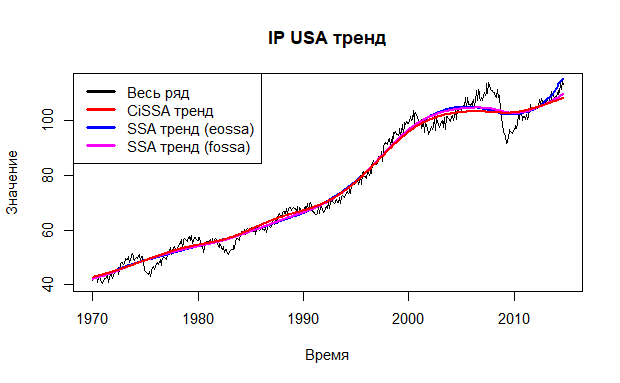
\includegraphics[width=1\textwidth]{img/trend inseparability example/IP_trend.png}
			\caption{Трендовая составляющая данных IP USA}
			\label{fig:IP_trend}
		\end{figure}
		
		\note{
			При применении FOSSA улучшения разделимости алгоритм $\SSA$ выделяет тренд довольно похоже с $\CISSA$. Весь график $\SSA$ тренд EOSSA выглядит более изогнутым при визуальном сравнении с остальными.
		}
		
		
	\end{frame}
	
	\begin{frame}{Сравнение алгоритмов. Реальные данные}
		\begin{figure}[H]
			\centering
			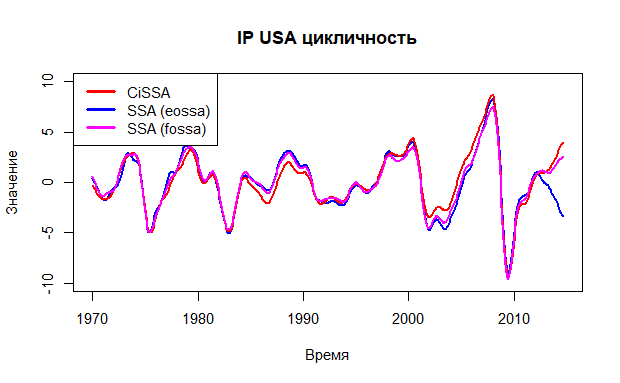
\includegraphics[width=1\textwidth]{img/trend inseparability example/IP_cycle.png}
			\caption{Циклическая составляющая данных IP USA}
			\label{fig:IP_cycle}
		\end{figure}
		
		\note{
			Аналогичная тренду ситуация происходит с цикличностью. В случае EOSSA правый хвост (значения ряда после 2010-ого года) смешался между цикличностью и трендом.
		}
		
		
	\end{frame}
	
	
	\begin{frame}{Сравнение алгоритмов. Реальные данные}
		\begin{figure}[H]
			\centering
			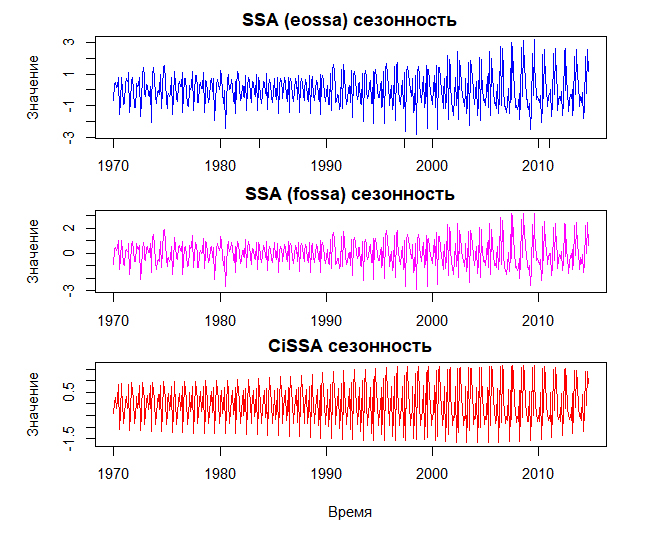
\includegraphics[width=0.8\textwidth]{img/trend inseparability example/IP_sesonal.jpg}
			\caption{Сезонная составляющая данных IP USA}
			\label{fig:IP_sesonal}
		\end{figure}
		
		\note{
			Поскольку в базовом $\SSA$ адаптивный базис, сезонность является менее систематичной, разброс значений выше по сравнению с $\CISSA$.
			
			Таким образом, получились довольно похожие результаты в выделении тренда и цикличности при использовании $\SSA$ с FOSSA и $\CISSA$. Несколько иные результаты при $\SSA$ с EOSSA. Сезонная составляющая в силу неадаптивного базиса более строго выглядит для метода $\CISSA$.
		}
		
		
	\end{frame}
	
	
	\begin{frame}{Заключение}
		По полученным результатам, можно следующие выводы: 
		\begin{enumerate}
			\item Алгоритм $\CISSA$ работает лучше разложения Фурье;
			\item Если понятно, что ряд состоит только из периодических компонент, стоит использовать $\CISSA$ без процедуры расширения, поскольку она делает ошибки разделений периодики больше. И напротив, если есть непериодичность, лучше расширять ряд;
			\item Если данные зашумлены или имеется непериодичность, алгоритм $\SSA$ с улучшением разделимости справляется в среднеквадратичном лучше $\CISSA$ с расширением ряда или без.
		\end{enumerate}
		
		\note{
			В данной работе исследован алгоритм $\CISSA$, сравнены методы $\CISSA$ и $\SSA$, и полученные
			знания были проверены на реальных и смоделированных примерах с помощью языка R. Оба алгоритма справляются с поставленными задачами, существенным различием является то, что алгоритм $\SSA$ является более гибким: в нем адаптивный базис, есть дополнительные алгоритмы, которые довольно похоже приближают этот алгоритм к $\CISSA$, а также методы для автоматического выбора компонентов по частотам. Метод $\CISSA$ является простым в использовании.
			
			Дальнейшими действиями является рассмотрение других модификаций метода $\SSA$.
			
			Все вычисления, а также код $\CISSA$ можно найти в github репозитории \citep{spbu_cissa_coursework_github}.
		}
		
		
	\end{frame}
	
	
	
	
	\begin{frame}{Список литературы}
		\small
		\bibliographystyle{plainnat}
		\bibliography{ref.bib}
		
		\note{
			На данном слайде представлен список основных источников, используемых в моей работе.
			Спасибо за внимание.
		}
	\end{frame}
	
\end{document}
